\documentclass[titlepage,11pt]{article}
\usepackage{graphicx,setspace,natbib,fancyvrb,geometry,rotating,capt-of}
\topmargin=-.2in\oddsidemargin=0pt\evensidemargin=0pt\textwidth=6.5in
\textheight=9in\headsep=.65in\headheight=0in
%\addtolength{\headheight}{2.5pt}

\begin{document}
\onehalfspace

\begin{singlespacing}
\title{Integrating a Heat Balance Equation}
\author{Cameron Bracken\\Humboldt State University\\ENGR 326}
\date{\today}
\maketitle
\newpage
\pagenumbering{roman}\pagestyle{myheadings}
\tableofcontents\addcontentsline{toc}{section}{List of Figures}
\listoffigures \addcontentsline{toc}{section}{List of Tables}
\listoftables
\newpage
\end{singlespacing}
\pagestyle{headings}\pagenumbering{arabic}

\section {Introduction}
One method used for heating a steady stream of ethylene glycol fluid
is a shell and tube heat exchanger (Figure \ref{fig:exchanger}). The
fluid is surrounded by a shell containing a saturated vapor which is
continuously condensed so that the temperature can be maintained at
$T_s$. The fluid has an inlet temperature of $T_1$ and an outlet
temperature of $T_2$.

\begin{figure}[h]\label{fig:exchanger}
\begin{center}
\scalebox{.7}{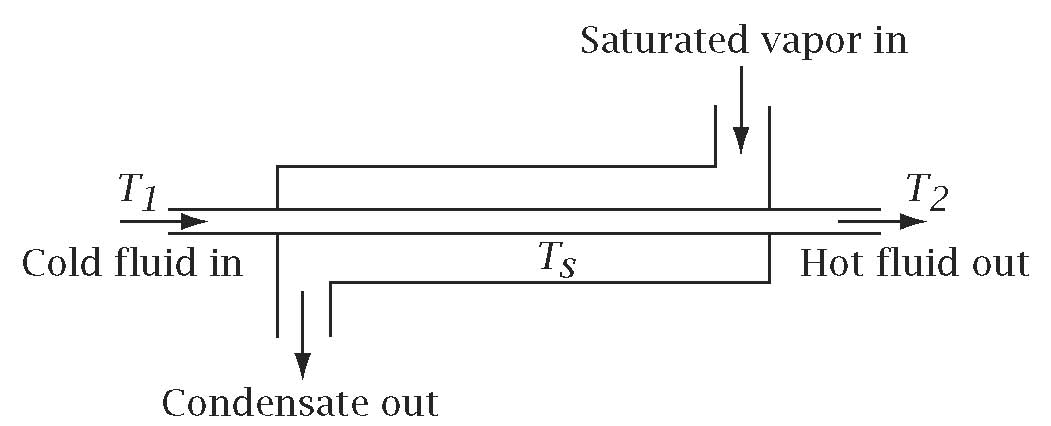
\includegraphics{exchanger.jpg}} \caption{Heat
exchanger}
\end{center}
\end{figure}
\noindent The length for the heat exchanger is found from a heat
balance differential equation (Finney 2006)
\begin{equation}\label{eq:heat}
\frac{dL}{dT}=\frac{m c_p}{\pi D h (T_s-T)^2}
\end{equation}
where
\begin{singlespacing}
\begin{center}
\begin{tabular}{rcl}
$m$&=&Mass flow rate (lb/hr)\\
$D$&=&Tube diameter (ft)\\
$\omega$ &=&Local heat transfer coefficient\\
$c_p$ &=&Specific heat of ethylene glycol
\end{tabular}
\end{center}
\end{singlespacing}
\noindent $\left(\ref{eq:heat}\right)$ is an integrable ODE so
integrating with respect to T gives L in terms of T
\begin{equation}\label{eq:int}
L=\frac{m }{\pi D}\int^{T_2}_{T_1}{\frac{c_p dT}{h (T_s-T)^2}}
\end{equation}
The local heat transfer coefficient is found from
\begin{equation}
h=\frac{0.023k}{D}\left(\frac{4m}{\pi D
\mu}\right)^{0.8}\left(\frac{\mu c_p}{k}\right)^{0.4}
\end{equation}
where
\begin{singlespacing}
\begin{center}
\begin{tabular}{rcl}
$k$&=&Thermal conductivity of ethylene glycol(BTU/hr$\cdot^\circ$F)\\
$\mu$&=&Viscosity (lb/ft$\cdot$hr)\\
\end{tabular}
\end{center}
\end{singlespacing}
Viscosity can be determined from the relationship
\begin{equation}
\ln{\mu}=.00002T^2-.0225T+5.4874
\end{equation}
Specific heat is given by the relationship
\begin{equation}
c_p=.053 + .00065T
\end{equation}
The values of $\mu$ and $c_p$ were determined by a polynomial fit of
experimental data (Finney 2006).

\section{Methodology}

To carry out the integration in (\ref{eq:int}) the function must be
in term of $T$.  Substituting the values of the parameters into
(\ref{eq:int}) results in a graph that has a parabolic shape (figure
\ref{fig:tvsl}).
\begin{figure}[h]\label{fig:tvsl}
  \begin{center}
    \scalebox{.4}{\includegraphics{TvsL.jpg}}
    \caption{The area under the graph represents pipe length(total area not shown)}
  \end{center}
\end{figure}

\noindent(\ref{eq:int}) has no easily attainable analytical solution
so a numerical method must be used to evaluate the integral.  In
this case the method of Romberg integration based on the trapezoid
rule is a sufficiently robust method.  A Romberg integration routine
combines an approximate integration technique (in this case the
trapezoid rule) with Richardson's improvement formula.  In each
iteration of a Romberg integration routine the step size is scaled
by some constant amount and then the new extrapolations are
computed.

The trapezoid rule for computing the approximate integral between
$a$ and $b$ has the general form
\begin{equation}
    \int^b_a{f(x)}=h\left[\frac{f(a)}{2}+\displaystyle\sum_{i=2}^{np}{f
    \left[a+(i-1)h\right]}+\frac{f(b)}{2}\right]
\end{equation}
where $h$ is the step size $([b-a]/np)$ and $np$ is the number of
panels to be used. When $np=1$ (i.e. the first iteration) the
trapezoid rule is very simple to program (figure
\ref{fig:traprule})(appendix A).
\begin{figure}[h] \label{fig:traprule}
\begin{center}
\begin{Verbatim}[frame=single]
  nt=1
  h=(b-a)/nt
  endpts=f(b)/(2d0)+f(a)/(2d0)
  area=(h)*(endpts)
\end{Verbatim}
\caption{First iteration of the trapezoid rule in a Romberg
integration routine}
\end{center}
\end{figure}

Richardson's improvement formula uses a weighted average of
approximate solutions (obtained using the trapezoid rule) with the
same error order to extrapolate a solution with a higher error
order.  The second approximation must have a different step size
than the first approximation. Richardson's improvement formula has
the general form
\begin{equation}
I_2(h_2)=\frac{r^kI_1(h_2)-I_1(h_1)}{r^k-1}
\end{equation}
where $h_1=rh_2$ and $r>1$. Program \verb heatex  combines the
trapezoid rule and Richardson's improvement formula to carry out the
integration in (\ref{eq:int})(figure \ref{fig:romberg}).

\begin{figure}[h] \label{fig:romberg}
\begin{center}
\begin{Verbatim}[frame=single]
  j=0
  do
    j=j+1
    h=h/r
    nt=2d0*nt
    do i=1,nt/2                !trapazoid rule
      newp=newp+f(a+(i-1)*(2d0*h)+h)
    end do
    IG(j+1,2)=(h)*(endpts+newp)
    k=1
    do i=1,j
      k=2*k                     !richardson's improvement
      IG(j+1,i+2)=((r**(k)*IG(j+1,i+1))-IG(j,i+1))/(r**(k)-1)
    end do
  end do
\end{Verbatim}
\caption{Romberg integration routine}
\end{center}
\end{figure}

\newpage The stopping criteria for program \verb heatex  are a solution
found test and a maximum iterations test (figure 5).

\begin{figure}[h] \label{fig:stop}
\begin{center}
\begin{Verbatim}[frame=single]
  if(j>maxit-2)then
      write(*,*)"Reached max iteration"
      numit=j
      return
    else if(tol<eps)then
      ans=IG(j+1,j+2)
      numit=j
      exit
      return
    end if
\end{Verbatim}
\caption{Stopping Criteria}
\end{center}
\end{figure}
\section{Application}

The pipe length in the heat exchanger is determined from various
parameters that are known in the problem (Table 1).

\begin{table}[h]
\begin{center}
\caption{Parameters associated with determining pipe length}
% Table generated by Excel2LaTeX from sheet 'Sheet1'
\begin{tabular}{|l|l|l|}
\hline
{\bf Parameter} & {\bf Variable} & {\bf Value} \\
\hline
Tube diameter  &        $D$ &      .086 ft \\
\hline
Vapor Temperature&      $T_s$ &      250 $^\circ $F \\
\hline
Mass flow rate  &        $m$ & 45000 lb/hr \\
\hline
Solution tolerance &        $\varepsilon$ &  $10^{-10}$ \\
\hline Specific heat & $c_p$ & J/lb$\cdot$F\\
\hline Viscosity & $\mu$ & lb/ft$\cdot$hr\\\hline
\end{tabular}
\end{center}
\end{table}

To test the sensitivity of the system, different parameters can be
varied (Table 2).

\begin{table}[h]
\begin{center}
\caption{Variation of Parameters}
% Table generated by Excel2LaTeX from sheet 'Sheet3'
\begin{tabular}{|c|r|r|r|r|}
\hline
{\bf Run \#} & {\bf Variable} & {\bf Initial value} & {\bf New value} & {\bf Variation} \\
\hline
         1 &     $D$ &     .086 ft &       .0774 &       -10\% \\


          2& &        .086 ft &       .0946 &       10\% \\

 \hline
         3 &  $T_s$ &        250 $^\circ $F &       225 &       -10\% \\


         4 &   &        250 $^\circ $F &       275 &       10\% \\

 \hline
         5 &  $m$ &        45000 lb/hr &       40500 &       -10\% \\


        6 &  &        45000 lb/hr &       49500 &       10\% \\

\hline
        7 &  $\varepsilon$ &        $10^{-10}$ &       $1\cdot10^{-5}$ &       -50\% \\


        8 &   &        $10^{-10}$ &       $1\cdot10^{-15}$ &       50\% \\

 \hline
9&$c_p$&no scale&.9 scale&-10\%\\
 10&$$&no scale&1.1 scale&10\%\\
\hline 11&$\mu$&no scale&.9 scale&-10\%\\
 12&$$&no scale&1.1 scale&10\%\\
\hline
\end{tabular}
\end{center}
\end{table}
\break

\section{Results}

With $T_2=90^\circ$F program \verb heatex  gives the pipe length
L=0.3967153601 (figure 6).

\begin{figure}[h] \label{Tlow}
\begin{center}
\begin{Verbatim}[frame=single]
The best estimate is:   0.3967153601
     # of iterations:   5

The Romberg extrapolation table is (first col. is stepsize):
       h             I 1           I 2           I 4           I 5
 90.0000000000  0.4157619924  0.0000000000...0.0000000000  0.0000000000
 45.0000000000  0.4016544622  0.3969519521...0.0000000000  0.0000000000
 22.5000000000  0.3979631260  0.3967326806...0.0000000000  0.0000000000
 11.2500000000  0.3970281530  0.3967164953...0.3967154059  0.0000000000
  5.6250000000  0.3967936117  0.3967154313...0.3967153601  0.3967153601
\end{Verbatim}
\caption{Abridged Romberg integration results for $T_2=90^\circ$}
\end{center}
\end{figure}

\noindent With $T_2=180^\circ$F program \verb heatex  gives the pipe
length L=1.1347906901 (figure 7).

\begin{figure}[h] \label{Thigh}
\begin{center}
\begin{Verbatim}[frame=single]
The best estimate is:   1.1347906901
     # of iterations:   6

The Romberg extrapolation table is (first col. is stepsize):
       h             I 1           I 2           I 5           I 6
 180.000000000  1.7446267397  0.0000000000...0.0000000000  0.0000000000
 90.0000000000  1.3316105678  1.1939385105...0.0000000000  0.0000000000
 45.0000000000  1.1905851943  1.1435767365...0.0000000000  0.0000000000
 22.5000000000  1.1493974712  1.1356682301...0.0000000000  0.0000000000
 11.2500000000  1.1384920326  1.1348568864...1.1348014657  0.0000000000
  5.6250000000  1.1357191620  1.1347948718...1.1347906901  1.1347906901
\end{Verbatim}
\caption{Abridged Romberg integration results for $T_2=180^\circ$}
\end{center}
\end{figure}
\newpage
The sensitivity analysis reveals how the pipe length  and number of
iterations change when the parameters are individually varied.  It
can be seen from the table that the pipe length is most sensitive to
a change in the shell temperature.  A change in the parameter
epsilon results in an almost negligible change in the pile length
but it has an effect on the number of iterations to find the
solution. The data applies when $T_2=180 ^\circ$F.  The data for
$T_2=90 ^\circ$F is not included because it shows similar trends.

\begin{table}[h]
\begin{center}
\caption{Parameters associated with determining pipe length}
% Table generated by Excel2LaTeX from sheet 'AcrD227'
\begin{tabular}{|r|r|l|l|l|l|l|}
\hline
{\bf Run \#} & {\bf Variable} & {\bf New value} & {\bf Percent varied} & {\bf Pipe Length} & {\bf Variation} & {\bf \# iterations} \\
\hline
         1 &        $D$ &     0.0774 &       -10\% &1.0430611141     &8.08\%&          6\\

         2 &            &     0.0946 &        10\% &1.2247005097     &7.92\%&          6 \\
\hline
         3 &      $T_s$ &        225 &       -10\% &1.8479438758     &68.8\%&          6  \\

         4 &            &        275 &        10\% &0.7907736591     &30.32\%&         6   \\
\hline
         5 &        $m$ &      40500 &       -10\% &1.1111284458      &2.09\%&         6   \\

         6 &            &      49500 &        10\% &1.1566295968      &1.92\%&         6  \\
\hline
         7 & $\varepsilon$ &1$\cdot10^{-5}$&       -50\% &1.1348014657 &$\sim$0\%&     5      \\

         8 &            &$\cdot10^{-15}$ &        50\% &1.1347904658   &$\sim$0\%&     7    \\
\hline
         9 &      $c_p$ &  .9 scale  &       -10\% &1.0652738588      &6.13\%&         6   \\

        10 &            & 1.1 scale  &        10\% &1.2015763597      &5.89\%&         6   \\
\hline
        11 &      $\mu$ &  .9 scale  &       -10\% &1.0879595981      &4.13\%&         6   \\

        12 &            & 1.1 scale  &        10\% &1.1788887985      &3.89\%&         6   \\
\hline
\end{tabular}
\end{center}
\end{table}

As the required output temperature ($T_2$) approaches 250$^\circ$F
the pipe length approaches infinity (figure 8). Further optimization
could be done to find the best pipe length for optimal fluid
heating.\break\newpage
\begin{figure}[h] \label{PvsT}
  \begin{center}
    \scalebox{.5}{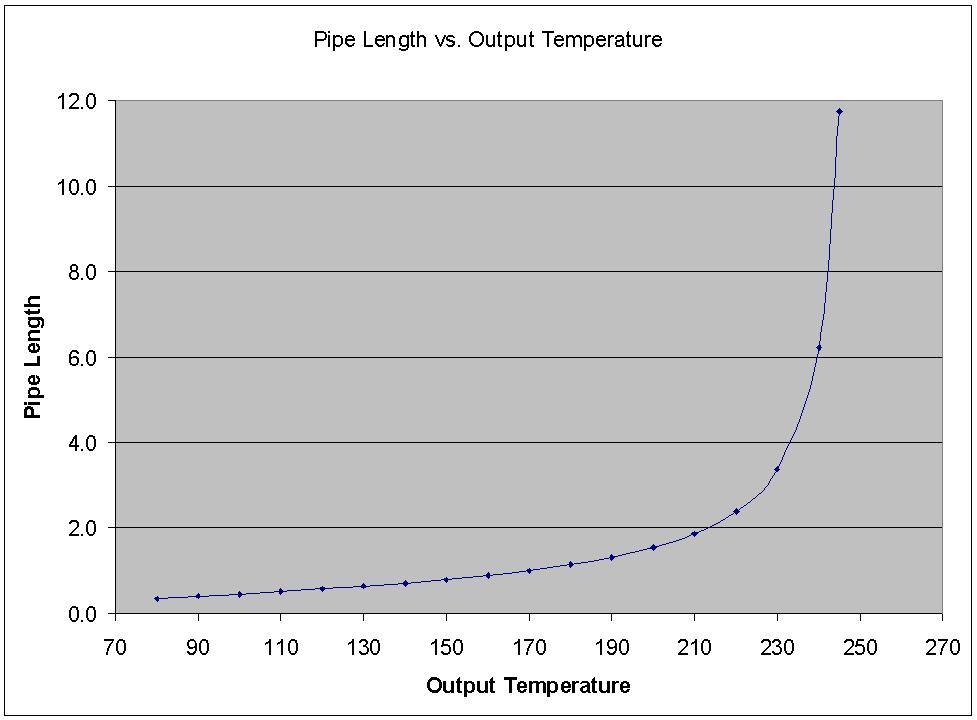
\includegraphics{PvsL.jpg}}
    \caption{($T_2$) approaches 250$^\circ$F as L approaches infinity}
  \end{center}
\end{figure}
\section{Conclusion}
The following can be concluded from the analysis:
\begin{itemize}
\item{The necessary pipe length when $T_2=90^\circ$F is L=0.3967153601}
\item{The necessary pipe length when $T_2=180^\circ$F is L=1.1347906901}
\item{Pipe length is most sensitive to a change in the shell temperature ($T_s$)}
\item{Required output temperature ($T_2$) approaches 250$^\circ$F as
the pipe length (L) approaches infinity.}
\end{itemize}

\section{References}
\noindent Finney,Brad. Lab 1 handout, Humboldt State University,
Spring 2006.

\appendix
\newcommand{\appsection}[1]{\let\oldthesection\thesection
  \renewcommand{\thesection}{Appendix \oldthesection}
  \section{#1}\let\thesection\oldthesection}
\appsection{\\~Source Code and Program Output} \label{sec:source}
\begin{singlespacing}
*Please note that the program output was slightly abridged in order
to fit them on one page.
\begin{Verbatim}[frame=single]
cwb12@ere-server:~/engr326/lab1> cat lab1.f90
module con
  double precision,parameter::e=2.718281828,pi=3.1415926,m=45000,D=.086,k=.153,
                              Ts=250
end module con

program heatex
  use con
  implicit none
  integer::numtrap,maxit,numit,s,j
  double precision::T1,T2,ans,eps
  character(len=30)::func
  double precision,allocatable,dimension(:,:)::I
  interface
    subroutine romtrap(nt,a,b,ans,maxit,eps,numit,IG,f)
      implicit none
      integer,intent(in)::nt,maxit
      integer,intent(out)::numit
      double precision,intent(in)::b,a,eps
      double precision,intent(out)::ans
      double precision,dimension(:,:),intent(out)::IG
      interface
        function f(x)
          double precision::x
          double precision::f
        end function f
      end interface
    end subroutine romtrap
    function temp(x)
      double precision::x
      double precision::temp
    end function temp
  end interface

    !this program will integrate a pre set flow equation using an integration
    !subroutine. The subroutine uses the trapezoid rule given upper and lower
    !limits, a number of trapezoids and a pipe radius.
    !variable list:
    !T1=lower limit of integration
    !T2=upper limit of integration
    !numtrap=number of trapezoids

  write(*,*)"This program will integrate an equation ",&
            "using a trapezoid rule integration subroutine(answer in feet)."
  write(*,*)"Enter the lower limit of integration."
  read(*,*)T1
  write(*,*)"Enter the upper limit of integration."
  read(*,*)T2
  numtrap=1
  !write(*,*)"Enter the number of trapezoids to use."
  !read(*,*)numtrap
  maxit=20
  allocate(I(maxit,maxit))
  eps=.0000000001
  call romtrap(numtrap,T1,T2,ans,maxit,eps,numit,I,temp)
  write(*,"(/,a,x,f14.10)")"The best estimate is:",ans
  write(*,"(5x,a,i4,/)")"# of iterations:",numit+1
  write(*,"(a)")"The Romberg extrapolation table is (first col. is stepsize):"
  write(*,"(7x,a,13x)",advance="no")"h"
  do j=1,numit+1
    write(*,"(a,i2,11x)",advance="no")"I",j
  end do
  write(*,"(a)",advance="yes")" "
  do s=1,numit+1
      write(*,"(100f14.10)")(I(s,j),j=1,numit+2)
  end do
  stop
end program heatex

subroutine romtrap(nt,a,b,ans,maxit,eps,numit,IG,f)
  implicit none
  integer,intent(inout)::nt,maxit
  integer,intent(out)::numit
  double precision,intent(in)::b,a,eps
  double precision,intent(out)::ans
  double precision,dimension(:,:),intent(out)::IG
  double precision::h,intp,endpts,newp,r,tol        !local variables
  integer::i,j,k

    !variable list:
    !h=        step size
    !a,b=      upper/lower limit of integration
    !interior= area under the curve without the endpoints
    !f=        function name

  interface
    function f(x)
      double precision::x
      double precision::f
    end function f
  end interface

  h=(b-a)/nt
    !write(*,*)h
  IG(1,1)=h
  intp=0
  do i=2,nt
    intp=intp+f(a+(i-1)*h)
  end do
  endpts=f(b)/(2d0)+f(a)/(2d0)
  IG(1,2)=(h)*(endpts+intp)

  r=2d0
  j=0
  do
    j=j+1
    h=h/r
    nt=2d0*nt
    IG(j+1,1)=h
    do i=1,nt/2
      newp=newp+f(a+(i-1)*(2d0*h)+h)
    end do
    IG(j+1,2)=(h)*(endpts+intp+newp)
    k=1
    do i=1,j
      k=2*k
      IG(j+1,i+2)=((r**(k)*IG(j+1,i+1))-IG(j,i+1))/(r**(k)-1)
    end do
    tol=abs(IG(j+1,j+2)-IG(j+1,j+1))
    if(j>maxit-2)then
      write(*,*)"Reached max iteration"
      numit=j
      return
    else if(tol<eps)then
      ans=IG(j+1,j+2)
      numit=j
      exit
      return
    end if
  end do

  return
end subroutine romtrap

function temp(T)
  use con
  double precision::temp,T,cp,lnu,u,ht
  cp=.53d0+.00065*T
  lnu=.00002d0*(T*T)-((.0225d0)*T)+5.4874d0
  u=e**(lnu)
  ht=((.023d0*k)/d)*(((4d0*m)/(pi*D*u))**(.8d0))*(((u*cp)/k)**(.4d0))
  temp=(m/(pi*D))*(cp/(ht*((Ts-T)**(2d0))))
  return
end function temp

cwb12@ere-server:~/engr326/lab1> ifort lab1.f90 -o lab1
cwb12@ere-server:~/engr326/lab1> lab1
 This program will integrate an equation
 using a trapezoid rule integration subroutine(answer in feet).
 Enter the lower limit of integration.
0
 Enter the upper limit of integration.
90

The best estimate is:   0.3967153601
     # of iterations:   5

The Romberg extrapolation table is (first col. is stepsize):
       h             I 1           I 2           I 3          I 5
 90.0000000000  0.4157619924  0.0000000000  0.0000000000...0.0000000000
 45.0000000000  0.4016544622  0.3969519521  0.0000000000...0.0000000000
 22.5000000000  0.3979631260  0.3967326806  0.3967180625...0.0000000000
 11.2500000000  0.3970281530  0.3967164953  0.3967154163...0.0000000000
  5.6250000000  0.3967936117  0.3967154313  0.3967153603...0.3967153601
cwb12@ere-server:~/engr326/lab1> lab1
 This program will integrate an equation
 using a trapezoid rule integration subroutine(answer in feet).
 Enter the lower limit of integration.
0
 Enter the upper limit of integration.
180

The best estimate is:   1.1347906901
     # of iterations:   6

The Romberg extrapolation table is (first col. is stepsize):
       h             I 1           I 2           I 3           I 6
 180.0000000000  1.7446267397  0.0000000000 0.0000000000...0.0000000000
 90.0000000000  1.3316105678  1.1939385105  0.0000000000...0.0000000000
 45.0000000000  1.1905851943  1.1435767365  1.1402192849...0.0000000000
 22.5000000000  1.1493974712  1.1356682301  1.1351409964...0.0000000000
 11.2500000000  1.1384920326  1.1348568864  1.1348027968...0.0000000000
  5.6250000000  1.1357191620  1.1347948718  1.1347907375...1.1347906901

\end{Verbatim}
\end{singlespacing}
\noindent This was typeset with \LaTeX
\end{document}
